\documentclass[sigconf]{acmart}
\usepackage{polyglossia}
\usepackage{booktabs} % For formal tables


% Copyright
%\setcopyright{none}
\setcopyright{acmcopyright}
%\setcopyright{acmlicensed}
%\setcopyright{rightsretained}
%\setcopyright{usgov}
%\setcopyright{usgovmixed}
%\setcopyright{cagov}
%\setcopyright{cagovmixed}


% DOI
\acmDOI{10.475/123_4}

% ISBN
\acmISBN{123-4567-24-567/08/06}

%Conference
\acmConference[WOODSTOCK'97]{ACM Woodstock conference}{July 1997}{El
  Paso, Texas USA}
\acmYear{1997}
\copyrightyear{2016}


\acmArticle{4}
\acmPrice{15.00}

% These commands are optional
%\acmBooktitle{Transactions of the ACM Woodstock conference}
\editor{Jennifer B. Sartor}
\editor{Theo D'Hondt}
\editor{Wolfgang De Meuter}


\begin{document}
\title{SIG Proceedings Paper in LaTeX Format}
\titlenote{Produces the permission block, and
  copyright information}
\subtitle{Extended Abstract}
\subtitlenote{The full version of the author's guide is available as
  \texttt{acmart.pdf} document}


\author{Ben Trovato}
\authornote{Dr.~Trovato insisted his name be first.}
\orcid{1234-5678-9012}
\affiliation{%
  \institution{Institute for Clarity in Documentation}
  \streetaddress{P.O. Box 1212}
  \city{Dublin}
  \state{Ohio}
  \postcode{43017-6221}
}
\email{trovato@corporation.com}

\author{G.K.M. Tobin}
\authornote{The secretary disavows any knowledge of this author's actions.}
\affiliation{%
  \institution{Institute for Clarity in Documentation}
  \streetaddress{P.O. Box 1212}
  \city{Dublin}
  \state{Ohio}
  \postcode{43017-6221}
}
\email{webmaster@marysville-ohio.com}

\author{Lars Th{\o}rv{\"a}ld}
\authornote{This author is the
  one who did all the really hard work.}
\affiliation{%
  \institution{The Th{\o}rv{\"a}ld Group}
  \streetaddress{1 Th{\o}rv{\"a}ld Circle}
  \city{Hekla}
  \country{Iceland}}
\email{larst@affiliation.org}

\author{Valerie B\'eranger}
\affiliation{%
  \institution{Inria Paris-Rocquencourt}
  \city{Rocquencourt}
  \country{France}
}
\author{Aparna Patel}
\affiliation{%
 \institution{Rajiv Gandhi University}
 \streetaddress{Rono-Hills}
 \city{Doimukh}
 \state{Arunachal Pradesh}
 \country{India}}
\author{Huifen Chan}
\affiliation{%
  \institution{Tsinghua University}
  \streetaddress{30 Shuangqing Rd}
  \city{Haidian Qu}
  \state{Beijing Shi}
  \country{China}
}

\author{Charles Palmer}
\affiliation{%
  \institution{Palmer Research Laboratories}
  \streetaddress{8600 Datapoint Drive}
  \city{San Antonio}
  \state{Texas}
  \postcode{78229}}
\email{cpalmer@prl.com}

\author{John Smith}
\affiliation{\institution{The Th{\o}rv{\"a}ld Group}}
\email{jsmith@affiliation.org}

\author{Julius P.~Kumquat}
\affiliation{\institution{The Kumquat Consortium}}
\email{jpkumquat@consortium.net}

% The default list of authors is too long for headers.
\renewcommand{\shortauthors}{B. Trovato et al.}


\begin{abstract}
This paper provides a sample of a \LaTeX\ document which conforms,
somewhat loosely, to the formatting guidelines for
ACM SIG Proceedings.\footnote{This is an abstract footnote}
\end{abstract}

%
% The code below should be generated by the tool at
% http://dl.acm.org/ccs.cfm
% Please copy and paste the code instead of the example below.
%
\begin{CCSXML}
<ccs2012>
 <concept>
  <concept_id>10010520.10010553.10010562</concept_id>
  <concept_desc>Computer systems organization~Embedded systems</concept_desc>
  <concept_significance>500</concept_significance>
 </concept>
 <concept>
  <concept_id>10010520.10010575.10010755</concept_id>
  <concept_desc>Computer systems organization~Redundancy</concept_desc>
  <concept_significance>300</concept_significance>
 </concept>
 <concept>
  <concept_id>10010520.10010553.10010554</concept_id>
  <concept_desc>Computer systems organization~Robotics</concept_desc>
  <concept_significance>100</concept_significance>
 </concept>
 <concept>
  <concept_id>10003033.10003083.10003095</concept_id>
  <concept_desc>Networks~Network reliability</concept_desc>
  <concept_significance>100</concept_significance>
 </concept>
</ccs2012>
\end{CCSXML}

\ccsdesc[500]{Computer systems organization~Embedded systems}
\ccsdesc[300]{Computer systems organization~Redundancy}
\ccsdesc{Computer systems organization~Robotics}
\ccsdesc[100]{Networks~Network reliability}


\keywords{ACM proceedings, \LaTeX, text tagging}


\maketitle

\section{Parsimony/parcimonie}

Le principe de parcimonie, principe \'{e}nonc\'{e} par Guillaume d'Occam, qui interdit
    de multiplier le nombre de choses \`{a} moins d'y \^{e}tre contraint. (Ce principe est \'{e}galement appel\'{e} rasoir d'Occam.)\cite{larousse01}.

\subsection{exemple parsimony}

\subsection{small and Large parsimony}
What are the small and large parsimony problems? Which one is harder? Why?

%http://www-master.ufr-info-p6.jussieu.fr/2005/IMG/pdf/L4_Arbres_Phylogenetiques_AAGB_IAD.pdf

%https://www.khanacademy.org/science/biology/her/tree-of-life/a/building-an-evolutionary-tree

%http://newprairiepress.org/cgi/viewcontent.cgi?article=1000&context=textbooks

\subsection{sankoff and ficth}
l'algorithme de sankoff et l'algorithme de ficth sont des algorithmes de reconstructions de arbres phylog\'{e}niques bas\'{e}e sur les caract\`{e}res.tous deux utilisent les fondements de la programmation dynamique pour r\'{e}soudre des probl\`{e}mes d'étiquettages d'arbres.
\subsubsection*{application}

Given  the  following  sequences,  topology and cost matrices,  apply the Fitch  and
Sankoff’s algorithms to calculate the scores

\paragraph{sankoff}
Soit la matrice de penalite de sankoff \\
\begin{table}[!h]
  \centering
\begin{tabular}{|l|c|c|c|r|}
\hline
    & A & T & G & C \\
  \hline
  A  & 0 & 3 & 4 & 9 \\
	\hline
	T  & 3 & 0 & 2 & 4 \\
	\hline
  G  & 4 & 2 & 0 & 4 \\
  \hline
  C  & 9 & 4 & 4 & 0 \\
  \hline
\end{tabular}
	\caption{Sankoff algorithm}
	\label{tab:commands}
\end{table}
\textcolor{red}{Todo}
\paragraph{fitch}

Soit la matrice de penalite de fitch \\
\begin{table}[!h]
  \centering
\begin{tabular}{|l|c|c|c|r|}
\hline
    & A & T & G & C \\
  \hline
  A  & 0 & 1 & 2 & 3 \\
	\hline
	T  & 1 & 0 & 2 & 4 \\
	\hline
  G  & 2 & 2 & 0 & 1 \\
  \hline
  C  & 3 & 4 & 1 & 0 \\
  \hline
\end{tabular}
	\caption{Fitch algorithm}
	\label{tab:commands}
\end{table}
\textcolor{red}{Todo}
\subsection{the nearest neighbor}

 What is the main idea of the nearest neighbor interchange algorithm?  Why it is
considered a heuristic method?

\section{Reconstruction using reversal distances}

\subsection{application web site Part 1}
Go to the web page \url{http://cinteny.cchmc.org} , choose human and mouse and click start. Then, select whole genome analysis (using human genome as reference).For human, genes are colored by chromosome, while for mouse by chromosome of human's homologous genes.  Include both figures in your report.

\begin{figure}[!h]
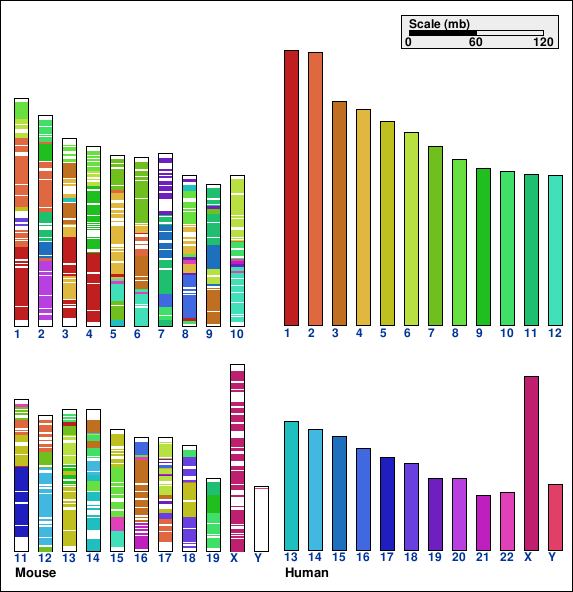
\includegraphics[width=8cm,height=8cm]{imag/graph1}
\caption{analyse du g\'{e}nome humain et de la souris chacun de fa\c{c}on entier }
\end{figure}

\subsection{application web site Part 2}
Start again with human and mouse but select chromosome versus chromosome
for chromosome 1 in human and 4 in mouse.  What is the reversal distance?  Why a big part of each chromosome was left in white?  Include the figure in your report.
\begin{figure}[!h]
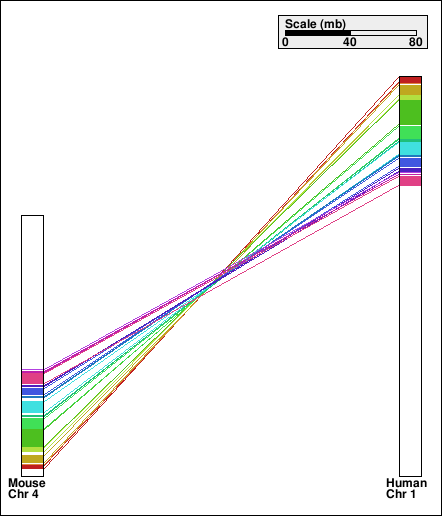
\includegraphics[width=8cm,height=8cm]{imag/graph2}
\caption{analyse du genome humain et de la souris sur des le chromosone 1 pour le genome Humain et le chromosone 4 pour la souris\texttt{includegraphics} command.}
\end{figure}

Mouse chr 4 - Human chr 1
Number of synteny blocks: 14
Reversal Distance: 1
Breakpoint Reuse: 1.00
\paragraph{whatis the reversal distance?}
la distance de reversal 
\textcolor{red}{Todo}

\subsection{application web site Part 3}
Now start again with human, mouse, cow, and chimpanzee. Choose a whole genome
analysis, write the matrix of reversal distances.  Include this matrix in your report.


Chimp-Human:
Number of synteny blocks: 723
Reversal Distance: 18
Breakpoint Reuse: 1.12

Cow-Mouse:
Number of synteny blocks: 1005
Reversal Distance: 360
Breakpoint Reuse: 1.54

Chimp-Mouse:
Number of synteny blocks: 957
Reversal Distance: 306
Breakpoint Reuse: 1.59

Chimp-Cow:
Number of synteny blocks: 990
Reversal Distance: 261
Breakpoint Reuse: 1.31

Mouse-Human:
Number of synteny blocks: 936
Reversal Distance: 302
Breakpoint Reuse: 1.61

Cow-Human:
Number of synteny blocks: 980
Reversal Distance: 257
Breakpoint Reuse: 1.31
\pgfplotsset{compat=newest}            % Permet l'affichage de deux axes y
 
\begin{figure}[!h]
\centering
\begin{subfigure}[b]{0.15\textwidth}
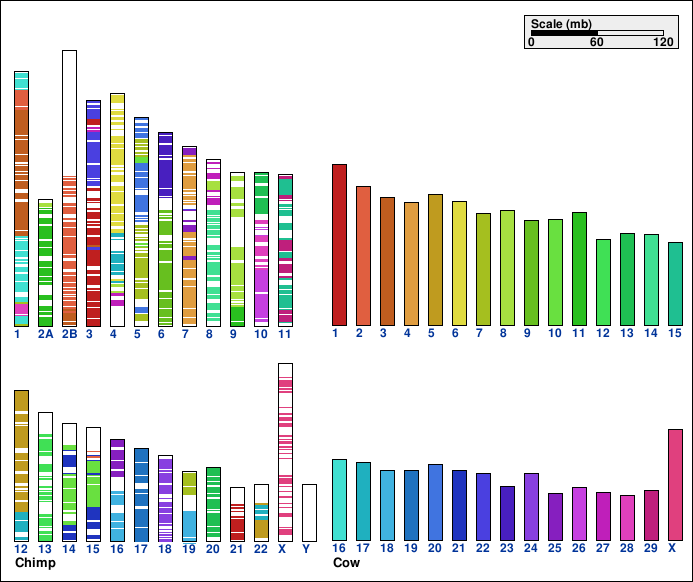
\includegraphics[width=\textwidth]{imag/graph3_chim_cow1}
\end{subfigure}
\begin{subfigure}[b]{0.14\textwidth}
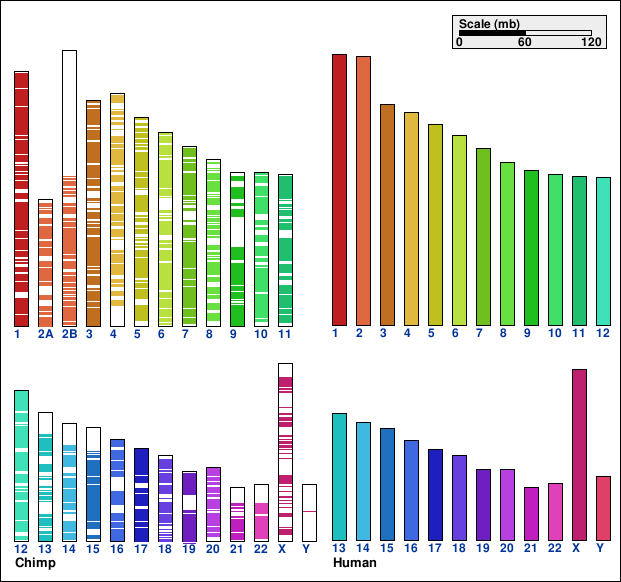
\includegraphics[width=\textwidth]{imag/graph3_chim_Himan1}
\end{subfigure}
\begin{subfigure}[b]{0.13\textwidth}
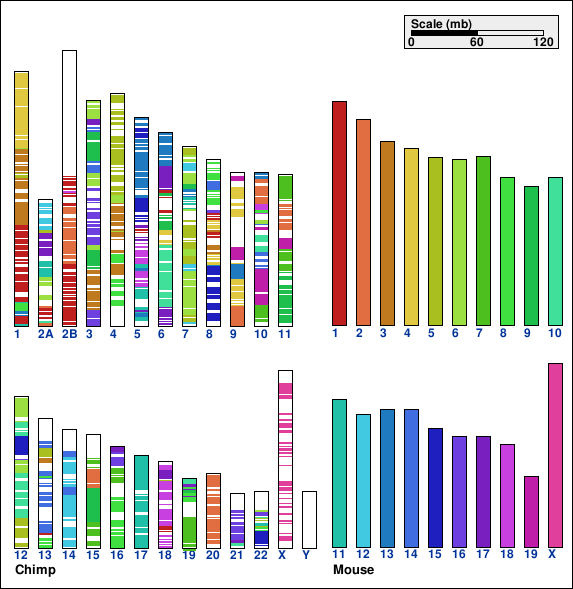
\includegraphics[width=\textwidth]{imag/graph3_chim_mouse1}
\end{subfigure}
\caption{3 images de r\'{e}sultats de comparaisons des genomes cow vs chimpanzee ;chimpanzee vs Himan; chimpanzee vs mouse}
\end{figure}
\begin{figure}[!h]
\centering
\begin{subfigure}[b]{0.15\textwidth}
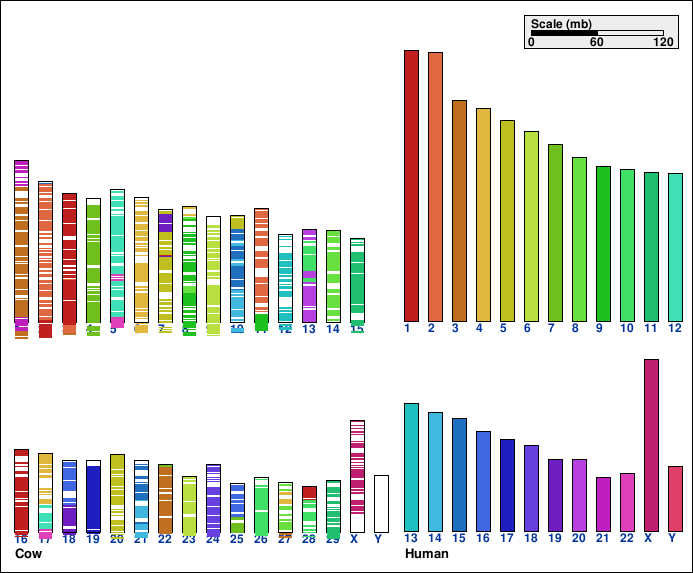
\includegraphics[width=\textwidth]{imag/graph3_cow_humain1}
\end{subfigure}
\begin{subfigure}[b]{0.15\textwidth}
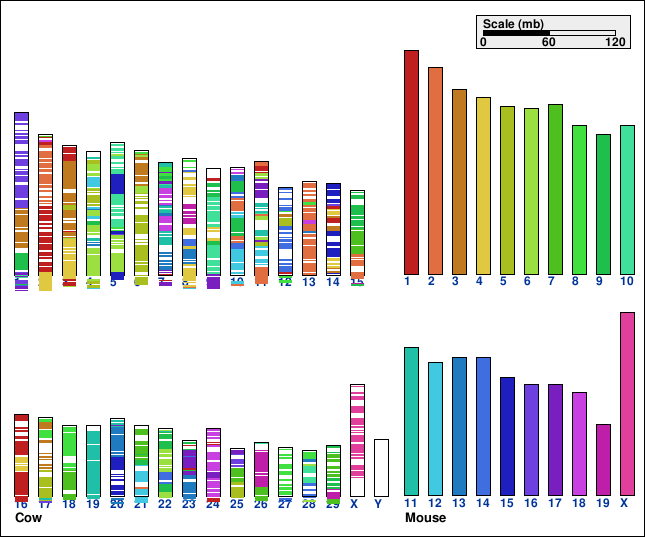
\includegraphics[width=\textwidth]{imag/graph3_cow_mouse1}
\end{subfigure}
\begin{subfigure}[b]{0.13\textwidth}
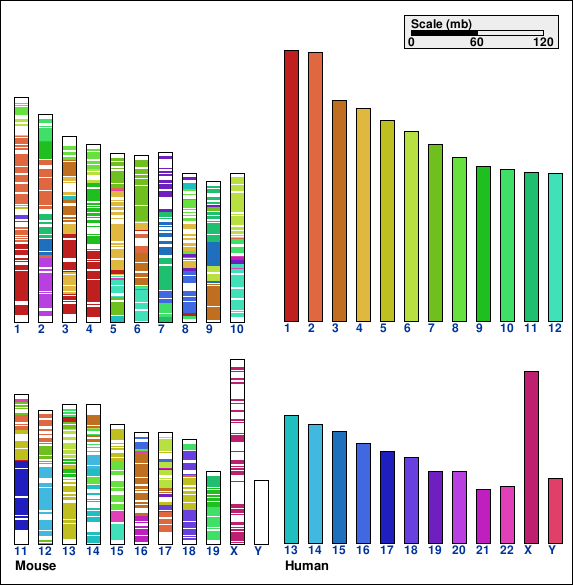
\includegraphics[width=\textwidth]{imag/graph3_mouse_Himan1}
\end{subfigure}
\caption{3 images de r\'{e}sultats de comparaisons des genomes cow vs humain ;cow vs mouse; mouse vs Humain}
\end{figure}

\begin{table}[!h]
  \centering
\begin{tabular}{|l|c|c|c|r|}
\hline
    & A & T & G & C \\
  \hline
  A  & 0 & 1 & 2 & 3 \\
	\hline
	T  & 1 & 0 & 2 & 4 \\
	\hline
  G  & 2 & 2 & 0 & 1 \\
  \hline
  C  & 3 & 4 & 1 & 0 \\
  \hline
\end{tabular}
	\caption{Fitch algorithm}
	\label{tab:commands}
\end{table}

\subsection{Using PHYLIP'S}
Use PHYLIP's command neighbor to compute NJ and UPGMA trees from this matrix.  Are these trees correct?

\bibliographystyle{ACM-Reference-Format}
\bibliography{sample-bibliography}

\end{document}
